% !TEX root = ../msc_thesis.tex

\chapter{Background}
\label{cha:background}

  \section{Passwords}
    \label{sec:passwords}
    Passwords are secret strings of characters which have been used as the primary method for both online and offline user authentication in the computing era. They appear in various forms and they are generally classified depending on their allowed character set and length. The term \emph{password} commonly refers to strings of small to average length (6-16 characters), while a \emph{passphrase} is usually a longer string (>20 characters), often a sequence of words. Alphanumeric characters are allowed in passwords and passphrases, and in many cases other ASCII printable characters are included in the available character sets. Passwords created for services often must abide by a \emph{password policy}, a set of requirements enforced by that individual service/organisation, in an effort to increase password strength and security~\cite{pass_policy,NIST_invalid}, as previous research has shown that in the absence of a password policy, users tend to select generally weaker and guessable passwords~\cite{reused_passwords,pass_policy_users_bad}.

    Ideally, passwords must comply with two conflicting requirements: they should be easy to remember and use without writing them down, while at the same time be unique for each service, look random and be hard to guess. This conflict is called the \emph{password problem} and is almost impossible for most users, experts and non-experts alike, who often reuse passwords or write them down to cope with it~\cite{the_password_problem,pass_management}. Komanduri et al. suggested the use of a password policy that is neither too stringent, but at the same time offers noticeable improvements in password strength.

    \subsection{Partial passwords}
      \label{ssec:partial_passwords}
      \emph{Partial password} was defined by D. Aspinall and M. Just~\cite{part_pass}:
      \begin{quote}
      A \emph{partial password} is a query of a subset of characters from a full password, posed as a challenge such as ``Give me letters 2, 3 and 6 from your password''.
      \end{quote}
      Throughout this dissertation we use a slightly different terminology; the term \emph{partial password challenge} is used to refer to such queries, and we use the term \emph{partial password} to refer to passwords on which \emph{partial password challenges} will be issued. The idea behind partial password challenges is that an adversary that observes a user answering the challenge (\eg by using a key-logger, a malware, or simply looking over the shoulder of the victim) will not be able to learn the whole password in one go.

      \subsubsection{Extent of partial password deployment}
        \label{sssec:partial_pass_extent_use}
        In 2012, Aspinall and Just collected and listed information about the authentication practices of 10 UK banks~\cite{2fa_uk}. In an attempt to refresh this information, we observed the publicly available demos and FAQs of the ``big four banks'' (a colloquial term, used to refer to the four largest banking groups), along with 3 more banks. All 7 examined financial institutions appeared to employ a partial password challenge as part of their authentication process. Partial passwords use was also encountered in some implementations of the \emph{3-D Secure} protocol for credit/debit card online transactions in Europe, such as the ``Verified by Visa'' and ``MasterCard SecureCode''.

        A similar approach, combined with a small-scale user survey on Amazon MTurk, indicated that this authentication scheme is uncommon in the US, as we were unable to detect a single bank that was using it.


  \section{Attacks on passwords}
    \label{sec:password_attacks}
    Several different methods of attacking passwords exist today (e.g. guessing attacks, dictionary attacks), and they are generally classified into one of the following categories, according to their origin.

    \subsection{Online attacks}
      \label{ssec:online_attacks}
      Online password attacks are performed over the internet, by attackers that attempt to guess a users' passwords. An important characteristic of such attacks is that they are usually rate-limited. Security-aware web services allow only a specific number of attempts of guessing a user's password before restricting or introducing delays for future attempts, as per the National Institute of Standards and Technology's (NIST) digital authentication guidelines~\cite{NIST}. Online attacks can be \emph{targeted}, aiming to get access to a specific user's account, or \emph{trawling}, attacking many different accounts and aiming to crack a portion of them. For instance, a trawling attack with 5\% success rate on 1000 bank accounts would manage to break into 50 of them (on average).

    \subsection{Offline attacks}
      \label{ssec:offline_attacks}
      Offline attacks on passwords are performed on stolen or leaked database dumps. The main differences between them and online attacks is that there is no limit on the number of attempts for a password; the only limits are the CPU and disk I/O speeds. Brute force searches for matches, cracking dictionaries and rule-based word mutation (mangling) are common techniques in the attempts to crack the passwords contained in the database. \emph{Unbound online attacks}, on web services that do not enforce an attempt limit, can use the aforementioned techniques, but produce results slower, due to the network delay introduced.


  \section{Password strength meters}
    \label{sec:pass_str_meters}
    A password strength meter is a Graphical User Interface (GUI) element that is displayed during password creation and offers visual feedback on the strength of the inputted password. Traditional strength meters have been the focus of previous research, regarding both their correctness and their effectiveness. As there is not yet a strict specification, different password meter implementations use different algorithms to measure a password's strength or guessability. Following a large-scale analysis of password meters in the wild, Castellucia et al. noted that great inconsistencies can be observed among them and that they often provide ``blatantly misleading'' strength measurements~\cite{pass_str_meter_analysis}.
    %TODO: Elaborate more "You might show a bulleted list of academic studies and their findings"

    \begin{figure}[H]
        \begin{subfigure}[t]{\textwidth}
            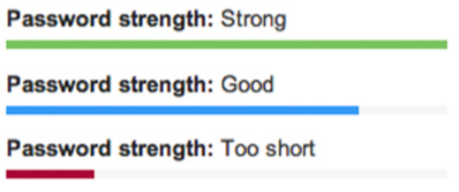
\includegraphics[width=0.5\textwidth]{Images/str-meter-google}
            \caption{Colored bar and text (Google)}
        \end{subfigure}

        \begin{subfigure}[t]{\textwidth}
            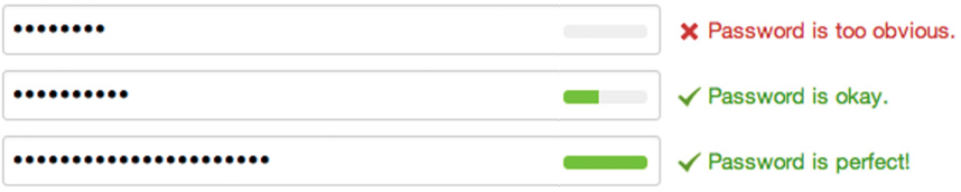
\includegraphics[width=\textwidth]{Images/str-meter-twitter}
            \caption{Green bar, text and checkmark (Twitter)}
        \end{subfigure}

        \begin{subfigure}[t]{\textwidth}
            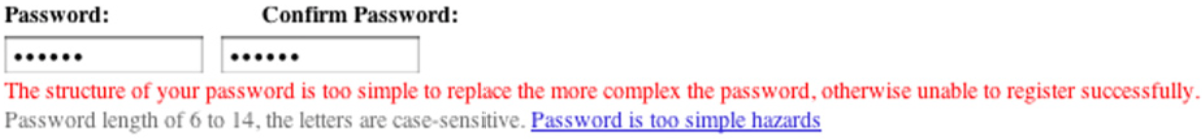
\includegraphics[width=\textwidth]{Images/str-meter-baidu}
            \caption{Text-only (Baidu)}
        \end{subfigure}

      \caption{Strength meter examples, taken from \cite{strength_meter_effect}}
      \label{fig:str_meter_examples}
    \end{figure}


  \section{Amazon Mechanical Turk (MTurk)}
    \label{sec:mturk}
    Amazon MTurk is a crowdsourcing platform that allows individuals to coordinate and solicit contributions from large groups of people for a wide range of human intelligence tasks (HITs). The platform is heavily used by academics for large-scale research that involves human subjects and it as been found to be a good source of high-quality data, while also achieving a better diversity in population demographics compared to an on-campus study~\cite{turk1,turk2}. Ipeirotis' analysis of MTurk demographics in 2010 indicated that workers are mainly from US and India, and, on average, younger and more technically adept than the general population\cite{mturk_demographic}.